\documentclass[sigconf,nonacm]{acmart}

\usepackage[textsize=small]{todonotes}

\bibliographystyle{alpha}
\title[Geodesic Paths and Distances]{Geodesic Paths and Distances\texorpdfstring{\\{\normalsize Report on \textit{A Survey of Algorithms for Geodesic Paths and Distances}}}{}}


\author{Matthieu Pierre Boyer}
\authornote{Both authors contributed equally.}
\affiliation{%
	\institution{École Normale Supérieure}
	\city{Paris}
	\country{France}}
\email{matthieu.boyer@ens.fr}

\author{Antoine Groudiev}
\authornotemark[1]
\affiliation{%
	\institution{École Normale Supérieure}
	\city{Paris}
	\country{France}}
\email{antoine.groudiev@ens.fr}

\def\abs#1{\left|#1\right|}
\def\R{\mathbb{R}}

\def\V{\mathbb{V}}
\def\nv{n_{\V}}
\def\E{E}
\def\ne{n_{\E}}
\def\F{\mathcal{F}}
\def\nf{n_{\F}}
\def\d{\mathrm{d}}

\begin{abstract}
	In this report, we investigate different methods to compute shortest-paths
	on meshed $2$-manifolds embedded in $\R^{3}$, based on \cite{craneSurvey}.
	We will most notably compare different types of methods, either coming from
	the resolution of PDEs on the manifold, or through the unfolding of the embedding to $\R^{2}$.
	We also provide from-scratch implementations of three methods, namely the heat method, fast marching, and the Improved Chen-Han algorithm, and compare their performances on several datasets.
	% for a blazingly fast™ result.
\end{abstract}

\begin{teaserfigure}
	% on peut remplacer l'image par quelque chose de plus horizontal du même genre, ou mettre plusieurs images côte à côte
	\centering
	\includegraphics[height=5cm]{images/rabbit-paths.png}
	\hspace{1cm}
	\includegraphics[height=5cm]{images/venus-paths.png}
	\hspace{1cm}
	\includegraphics[height=5cm]{images/star-paths.png}
	\caption{Geodesic paths on meshes, computed with our implementation of the Improved Chen-Han algorithm. Faces are colored from red to green according to the distance of their barycenter to the source point. The geodesic path to each vertex is drawn in blue.}
	\Description{}
	\label{fig:teaser}
\end{teaserfigure}

\begin{document}
\maketitle

\section*{Introduction}
Computing the distance between two points and retrieving a shortest path is, in general, a fundamental problem in computer science. While the problem is well understood in flat, Euclidean spaces, it becomes more challenging when considering curved surfaces.

\textcolor{red}{TODO: mathematical problem formulation in general}

Such a problem arises in various fields, including computer graphics, robotics, medical imaging, and computer vision. In computer graphics, geodesic distances are used for texture mapping \cite{oliveira2010geotextures}; in robotics, they form the cornerstone of path planning algorithms on complex terrains \cite{garrido2013application}; in medical imaging, they assist in analyzing anatomical structures \cite{miller2006geodesic}; and in computer vision, they improve object recognition and shape analysis \cite{shamai2017geodesic}.

The ability to efficiently compute geodesic distances and paths is therefore crucial for many applications in which the size of the problem is large, and where real-time performance is required. In the polyhedral setting, where the surface is represented as a mesh of vertices, edges, and faces, the number of vertices is derived from the desired accuracy of the representation, and can thus be very large. Algorithms with a low theoretical and practical complexity are therefore essential to handle such large-scale problems.

After brief mathematical reminders in \autoref{sec:math-reminders}, we present two methods based on the resolution of Partial Differential Equations (PDEs) in \autoref{sec:pde-methods}.
Then, in \autoref{sec:comp-geom-methods}, we discuss computational geometry methods, focusing on the Improved Chen-Han algorithm.
Finally, we present experiments and results in \autoref{sec:experiments}, and conclude in the final section.

\section{Mathematical reminders}
\label{sec:math-reminders}
Formally, a $2$-manifold (without boundary) is a topological space in which all points have neighborhoods homeomorphic
to disks (without boundary) in $\R^{2}$.
Intuitively, this means that zooming enough on any point of the manifold will make it look like a flat surface.
In \autoref{fig:manifolds-examples}, we can see that some meshes are not manifolds, as some points are locally non-flat.

\begin{figure}[ht]
	\centering
	\includegraphics[width=.4\linewidth]{images/manifold.png}
	\includegraphics[width=.5\linewidth]{images/nonmanifold.png}
	\caption{Examples of a $2$-manifold (left) and non-manifold (right) mesh. (Images generated from our custom viewer.)}
	\Description{}
	\label{fig:manifolds-examples}
\end{figure}

In our context, we will be given a $2$-manifold already meshed%
\footnote{\cite{craneSurvey} gives a few methods to create such a meshing. In particular, our implementations of the methods are restricted without loss of generality to triangular faces; more general meshes can be considered through triangulation techniques.}%
, that is, a finite set $\V \subseteq \R^{3}$ of vertices
(of cardinal $\nv$) and a finite set $\F \subseteq \left\llbracket 1, \nf\right\rrbracket^{3}$
of faces, given by the indices of the associated vertices.
The edges $\E$ of the manifold are given by any subsets of size two of a face $f \in \F$.
Because continuous functions on the manifold cannot be fully represented in memory, and especially by a
finite number of points on the mesh, functions on the manifold will be approximated by functions
on $\V$, on $\E$ or on $\F$.
As such, we will take any function and interpolate it linearly on each face, giving us a piecewise-linear
function.

A path on a piecewise-linear manifold can then be understood as interpolating on pieces of the manifold, or
directly computing the curves on the mesh.
The quality of the approximation by the mesh of the $2$-manifold will never be taken into account in the
quality results.

\section{PDE-based methods}
\label{sec:pde-methods}
In this section we will study methods inspired by Partial Differential Equations (PDE) that arise from models
of physical phenomena.
Indeed, many physical phenomena propagate along the surfaces over time, and dissipate over space, thus
allowing us to retrieve geodesics from solutions to the equations.

\subsection{General Theory}
Consider the parabolic heat equation
\begin{equation*}
	\frac{\d}{\d t}u_{t} = \Delta u_{t}.
\end{equation*}
Here, $u_{t}$ is the temperature profile at time $t$ and $\Delta$ is the laplacian operator (or divergence of the gradient operator).
However, on a piecewise-linear manifold, because functions on vertices are interpolated linearly to become
functions on the manifold, the gradient is piecewise-constant and can be computed explicitly from the
values at each vertex.
Consider a face $f \in \F$ with vertices $p_{i}, p_{j}, p_{k} \in \R^{3}$.
Let $e_{1} = p_{j} - p_{i}$ and $e_{2} = p_{k} - p_{i}$.
The face normal is
\begin{equation*}
	\overrightarrow{n_{f}} = \frac{e_{1} \times e_{2}}{\abs{e_{1} \times e_{2}}},
\end{equation*}
where $\times$ is the cross product in $\R^{3}$
and thus the gradient, being perpendicular to level curves is
\begin{equation}
	\nabla u_{\mid_{f}} = \frac{1}{2A_{f}}\sum_{l \in f}u_{l}(\overrightarrow{n_{f}}\times e_{l}), \label{eq:facegrad}
\end{equation}
where $A_{f} = \frac{1}{2}\abs{e_{1} \times e_{2}}$ is the area of face $f$ and $e_{l}$ is the \textbf{opposite} to vertex $l$.
Note that we can represent the gradient as a matrix $G \in \R^{\nv \times 3\nf}$, although this
representation is really inefficient for practical computation.
The definition of the divergence then comes from the Gauss-Ostrogradski theorem by intregration by parts
\begin{equation}
	\left(\nabla \cdot X\right)_{i} = \frac{1}{A_{i}}\sum_{f \ni i}\sum_{e \in f}\frac{1}{2}\cot{\left(\alpha_{e}^{f}\right)}\langle X_{f}, e\rangle, \label{eq:divergence}
\end{equation}
where $A_{i}$ is the Voronoi area associated with vertex $i$ and $\alpha_{e}^{f}$ is the angle at the vertex
opposite to edge $e$ in $f$.

Finally, we can define the Laplace-Beltrami operator (the piecewise-linear version of the continuous laplacian) as $\Delta = (\nabla \cdot) \circ \nabla : \V \to \R$ or simply
\begin{equation}
	(\Delta u)_{i} = \frac{1}{2A_{i}}\sum_{e = (i, j)}\left(\cot \alpha_{i, j} + \cot \beta_{i, j}\right)\left(u_{i} - u_{j}\right),\label{eq:laplacian}
\end{equation}
where $\alpha_{i, j}, \beta_{i, j}$ are the two angles opposite edge $(i, j)$.
One could then see the Laplace-Beltrami operator as a matrix $L \in \R^{\nv \times \nv}$.

\smallskip

After the spatial discretization of the laplace operator we just described, operating a time discretization in a single
backward Euler step for some fixed time $t$ will give us approximate solutions to the equation.
If we want to find the distance maps from some set $X \subseteq \V$, we simply solve the linear equation
associated to the continuous equation we need to solve.

\subsection{Physical Equations}
In our implementation, we compared multiple methods based on physical phenomena allowing to trace geodesics,
or at least geodesic-like curves.
Indeed, not all of those compute the true geodesic distance, but some sense of distance that can be drawn
and integrated to find shortest paths.

\paragraph{Heat Method}
This method is based on the heat equation
\begin{equation}
	\nabla u_{t} = \frac{\d}{\d t}u_{0},\label{eq:heat}
\end{equation}
which models the
evolution of temperature profiles $u_{t}$ in time in a given material, which here will be our surface,
from the initial profil $u_{0}$.
It can be derived
We discretize it as:
\begin{equation}
	(\mathrm{id} - t\Delta)u_{t} = u_{0}.\label{eq:discrheat}
\end{equation}
Retrieving the true geodesic distance can then be done by first normalizing the gradient
$X = -\nabla u_{t}/\abs{\nabla u_{t}}$ of the solution of the above equation that points along geodesics,
then solving the Poisson equation $\Delta \phi = \nabla \cdot X$ to retrieve the true distance function.
This fact comes from the Varadhan formula $\phi(x, y) = \lim_{t \to 0}\sqrt{-4t \log k_{t, x}(y)}$.

\cite{Crane:2017:HMD} suggest that the proper value of $t$ to use for computations here is around $h^{2}$
with $h$ the mean spacing between adjacent nodes, as $h\Delta$ is invariant with respect to scale.

\paragraph{Poisson Equations}
The equations in this paragraph all allow to draw geodesics-like curves, although they do not give the
actual metric on the manifold.
They are all based on the Poisson equation
\begin{equation}
	\Delta u = u_{0},\label{eq:poisson}
\end{equation}
which can be derived, for example, from the Maxwell equations to compute the electrostatic potential
along a charge distribution, or from the momentum equation to compute the pressure in an incompressible
fluid given its velocity.
% TODO: implement and provide informations


\paragraph{Wavefront Propagation}
The hyperbolic wavefront propagation equation (or d'Alembert equation)
\begin{equation*}
	\frac{\d^{2}}{\d t^{2}}u_{t} = c^{2}\Delta u_{t}, \text{or}, \square u = 0
\end{equation*}
where $\square$ is the d'Alembert operator, models the propagation of a wave in a material,
which will again be our surface here.
It arises for example the response of the surface to some elastic deformation $u$ (say, a stone dropping in
a pond) considering the stress tensor $T = E\nabla u$ with $E$ the homogenous modulus of elasticity (here,
the surface tension of the water) and considering the inertial force
$\rho \frac{\partial^{2}u}{\partial t^{2}}$ caused by the local acceleration (the stone moving the water
down on impact).

However, while retrieving distance information from Equations \eqref{eq:heat} and \eqref{eq:poisson} is
not too difficult and doable by solving a simple linear system, retrieving distance from propagating
wavefronts is more easily done from the non-linear hyperbolic eikonal equation
\begin{equation}
	\begin{cases}
		\abs{\nabla u}^{2} = 1 & \text{on } M,         \\
		u = 0                  & \text{on }\partial M,
	\end{cases}\label{eq:eikonal}
\end{equation}
which directly characterizes the distance to the boundary $\partial M$ (which in our case will be the set
we're computing the distance to).
The eikonal equation arises as the fundamental equation specifying the light paths in space given the
refractive index function of the media encountered.
In our case, there is a unique medium to be considered, and light sources $\partial M$ that emit the light.

\subsection{Implementation Details}
Our input manifold is given as a triangular mesh, that is a set $\V$ of vertices of $\R^{3}$ and a set
$\F \subseteq \left\llbracket 1, \abs{\V}\right\rrbracket^{3}$ of faces passed by indices.
We are also given a set $\partial M$ of sources or boundaries which will be points we compute the distance
to (or from).

\subsubsection{Linear equations}
In the case of linear equations such as Equations \eqref{eq:heat} and \eqref{eq:poisson}, we only have to
construct and solve a linear system of equations from the manifold and the set of sources:

\begin{itemize}
	\item We compute the gradient for the manifold and a function $u$ using the formula of Equation
	      \ref{eq:facegrad}, as the dynamic array of the face vectors.
	\item We also compute the laplacian operator for the manifold as the $\nv \times \nv$ matrix using
	      the cotangent formula of Equation \eqref{eq:laplacian} by iterating on all faces to iterate
	      on all edges and thus all vertices in the end.
	\item We discretize in time the equation with a single step of backwards Euler method and solve the
	      induced linear system, as done in Equation \eqref{eq:discrheat}.
\end{itemize}

For the heat equation, we can also retrieve approximate geodesics passing through vertices by solving
in $\phi$ the Poisson equation $\Delta \phi = \div X$ on the normalized gradient $X$ of the temperature
profile.
This is done by simply computing the divergence operator on the manifold from Equation \ref{eq:divergence},
and iterating on the faces to fill the divergence matrix of the manifold and solving another linear system.

\subsubsection{Fast Marching Method}
While the simple linear system solving works directly for the heat equation, solving for the geodesic paths
arising from the eikonal equation \eqref{eq:eikonal} is more difficult, as the equation is non-linear and
thus easy system resolution techniques will not work.

To work around this issue, we implemented the fast marching method, based on \cite{kimmelsethian}.
The method initializes the distance at the sources $\partial M$ to $0$ and iterates using a priority queue
on the neighbours of the already seen points.
The distances are not interated according to paths along edges, but so that the eikonal equation is
verified.
If we know values $\phi_{i}, \phi_{j}$ at two corners, we pick $\phi_{k}$ so that the slope of the triangle
$(i, j, k)$ for $\phi$ (so the norm of the gradient of $\phi$, $\left\lVert\nabla \phi\right\rVert$) is $1$.

\subsubsection{Limitations}
\paragraph{Linear PDEs}
The main issue that arises with the linear PDEs we consider is numerical stability.
Indeed, the laplacian of a manifold will usually be singular, so we need to add regularization terms at
every linear system resolution.
This yields a lot of numerical artifact when the discretization steps are too big for the precision we
can compute.
Moreover, while the method is polynomial, it scales quite poorly as the number of vertices increases, the
algorithm being in $\mathcal{O}(\nv^{3})$.

\paragraph{Fast Marching}
For the fast marching algorithm, the method is much shorter, as it runs in $\mathcal{O}(\nv \log \nv)$, but
this comes at the cost of stability when considering too small angles.
Indeed, the order in which vertices are updated might violate the causality property of the propagation.
Indeed, if triangles have obtuse angles, there might be point $i$ being closer to the source than another
point $j$ but the distance in $j$ might be finalized before the distance at $i$.
A solution to this exists but might not terminate due to its non-locality.

\section{Computational Geometry methods}
\label{sec:comp-geom-methods}
While PDE-based methods provide a general framework to compute geodesic distances on arbitrary, possibly non-meshed manifolds, we can leverage the fact that our manifold is meshed to design more efficient algorithms.
A whole class of such algorithms, arising from computational geometry, can be classified according to two main caracteristics.

\paragraph{Global vs.~local} Global methods compute globally optimal paths, up to numerical precision. Local methods start from an initial non-geodesic path and iteratively improve it until convergence to a local minimum.
\paragraph{Exact vs.~approximate} Exact methods compute the exact geodesic distance, while some approximate methods trade accuracy for speed, and compute only an approximation of the geodesic distance within some guaranteed error bound.
\vspace{5pt}

In the following, we focus on a global and exact method, the Improved Chen-Han algorithm \cite{chen1990shortest,xin2009improving}.

\subsection{Continuous Dijkstra}
The Improved Chen-Han (ICH) algorithm is based on the continuous Dijkstra paradigm introduced by Mitchell et al. for the Mitchell-Mount-Papadimitriou (MMP) algorithm \cite{mitchell1987discrete}.
The main idea is to apply Dijkstra's algorithm in the continuous setting of a piecewise-linear manifold.

A first natural approach could be to consider the graph formed by the vertices and edges of the mesh, and run Dijkstra's algorithm on it. However, this would only yield paths that follow the edges of the mesh, which can be arbitrarily longer than the true geodesic paths on the surface (see \autoref{fig:suboptimal-dijkstra}).

\begin{figure}[ht]
	\centering
	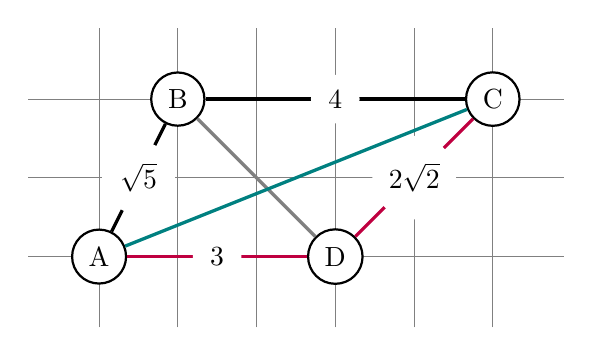
\begin{tikzpicture}
		\draw[step=1.0,gray,thin] (-0.9,-0.9) grid (5.9,2.9);

\begin{scope}[every node/.style={circle,thick,draw,fill=white}]
    \node (A) at (0,0) {A};
    \node (B) at (1, 2) {B};
    \node (C) at (5, 2) {C};
    \node (D) at (3, 0) {D};
\end{scope}

\begin{scope}[>=,every node/.style={fill=white,circle},every edge/.style={draw=black,very thick}]
    \path [->] (A) edge node {$\sqrt{5}$} (B);
    \path [->] (B) edge node {$4$} (C);
    \path [->] (B) edge[draw=gray] (D);
    \path [->] (A) edge[draw=purple] node {$3$} (D);
    \path [->] (D) edge[draw=purple] node {$2\sqrt{2}$} (C);
    
    \path [->] (A) edge[draw=teal] (C);
\end{scope}
	\end{tikzpicture}
	\caption{Example of suboptimality of applying Dijkstra's algorithm on the graph formed by the vertices and edges of the mesh. The red path follows the edges of the mesh, while the blue path is the true geodesic path on the 2D surface, which is shorter.}
	\Description{}
	\label{fig:suboptimal-dijkstra}
\end{figure}

Instead, we would like to consider each point on the surface as a potential node in the graph.
However, since the shortest path on a single face is always a straight line, it is sufficient to only consider points on the edges of the mesh as potential nodes.
This still yields an infinite number of potential nodes; a key concept of the MMP algorithm is to use instead a data structure called \textit{windows}, which encapsulate a continuous interval of points on an edge, along with the information needed to propagate the shortest path from these points to adjacent faces.

Formally, a window
\begin{equation*}
	w = (s, p, e, b_0, b_1, d_0, d_1, \sigma)
\end{equation*}
is defined on edge $e$, between points $b_0$ and $b_1$ (see \autoref{fig:ich-windows}). The window represents shortest paths originating from a ``pseudosource'' $p$, at a distance $\sigma$ from the actual source $s$. Distances from $p$ to the endpoints $b_0$ and $b_1$ of the window, respectively $d_0$ and $d_1$, are also stored.

\begin{figure}
	\centering
	\includegraphics[width=\linewidth]{images/window-illustration.png}
	\caption{{\textcolor{red}{TODO: tikzfy.}} Illustration of a window $w=(s, p, e, b_0, b_1, d_0, d_1, \sigma)$.}
	\Description{}
	\label{fig:ich-windows}
\end{figure}

\subsection{Window management and pruning}
While all revolving around the same core idea of continuous Dijkstra, different algorithms differ in how they manage and propagate windows \cite{craneSurvey}.

The original MMP algorithm does not perform aggressive pruning of windows, but trim overlapping windows on the same edge to avoid redundancy later on.
It uses a priority queue to always propagate the window with the smallest minimum distance first, ensuring both global optimality and early trimming of redundant windows.
\begin{figure}[ht]
	\centering
	\includegraphics[width=.4\linewidth]{example-image-b}
	\caption{Window trimming in the MMP algorithm.}
	\Description{}
	\label{fig:window-trimming}
\end{figure}

To achieve a better theoretical complexity, the Chen-Han algorithm substitutes the priority queue with a First-In-First-Out (FIFO) queue, propagating windows in the order they were created. To speed up the algorithm in practice, a pruning rule called ``one angle, one split'' is introduced; however, overlapping windows are not trimmed.

The Improved Chen-Han algorithm combines both approaches, using a priority queue to always propagate the window with the smallest minimum distance first, while also employing the ``one angle, one split'' pruning rule from Chen-Han. The pruning strategy is extended to trim overlapping windows on the same edge as well.

\begin{figure}[ht]
	\centering
	\includegraphics[width=.4\linewidth]{example-image-c}
	\caption{Extended ``one angle, one split'' pruning rule in the Improved Chen-Han algorithm.}
	\Description{}
	\label{fig:one-angle-one-split}
\end{figure}

\subsection{Algorithm outline and example}
We know give a high-level outline of the Improved Chen-Han algorithm, and illustrate it on a toy example.

\textcolor{red}{TODO}


\subsection{Implementation details}
We implemented the Improved Chen-Hand algorithm from scratch in Rust, following the description from \cite{xin2009improving}.
We provide here a short description of some implementation details, data structures used, as well as some difficulties we encountered and limitations of our implementation.

\subsubsection{Data structures}
As other methods, the input of the algorithm is a $2$-manifold represented as a triangle mesh, that is a set of vertices $\V$ and a set of faces ($3$-tuples) $\F$.
However, we also need to represent edges $\E$ explicitly, as windows are defined on edges. We therefore employ an edge data structure, storing for each edge both geometric information (length) and topological information (adjacent faces, vertices, \dots).
Notably, we precompute the twin edges for each edge, which is repeatedly invoked during window propagation.

The main algorithm relies on a priority queue of windows, ordered by the minimum distance from the source to any point in the window.
We implement this priority queue as a binary heap, using Rust's standard library implementation.
Windows are represented as structs containing all the necessary information for propagation, as described above.
Information about the vertices, such as the edge from which the shortest path to the vertex originates, is also stored during the main loop of the algorithm to enable path reconstruction later on.

\subsubsection{Limitations}
Two main limitations of our implementation are worth mentioning: paths along the edges fail to be computed successfully, and some vertices may not receive a distance value at the end of the algorithm when the geometry is particularly complex.

\section{Experiments and results}
\label{sec:experiments}
\textcolor{red}{TODO: do experiments, provide results, compare methods.}

\textcolor{red}{TODO: highlight the limitations of each method, and the tradeoffs.}

\subsection{Methodology}
We collected a set of \textcolor{red}{TODO: number} meshes of various sizes, ranging from \textcolor{red}{TODO: min} to \textcolor{red}{TODO: max} vertices.
Mesh come from various sources, including the Thingi10k dataset \cite{zhou2016thingi10kdataset100003dprinting}, filtered to only contain manifolds with a single connected component.
Each mesh was processed by our implementation of each method, starting from a single source vertex chosen arbitrarily.
For each mesh, each algorithm is run \textcolor{red}{TODO: number} times with different source vertices, the points in \autoref{fig:ich-experiments-results} corresponding to the average runtime over these runs.

Care should be taken when interpreting the following results, as the runtime depends on the specific geometry of the meshes used in the benchmark, and may not generalize to all possible meshes. 
The number of vertices is not always a fair indicator of the complexity of the geometry, and other factors such as the distribution of vertex valences and curvature may also impact the practical runtime of the algorithm.

\subsection{Runtime of linear PDE methods}
\subsection{Runtime of Fast Marching}

\subsection{Runtime of the ICH algorithm}
Theoretically, the Improved Chen-Han algorithm runs in $\mathcal{O}(n^2 \log n)$ time on a mesh with $n$ vertices, which is worse than the $\mathcal{O}(n^2)$ previously obtained by the Chen-Han algorithm, the $\log n$ factor coming from the priority queue management.

\cite{craneSurvey} reports that in practice, the ICH algorithm runs in sub-quadratic time on average, and dramatically improves the performance of the original Chen-Han algorithm, without supporting such a claim with a precise benchmark. We therefore conducted experiments to benchmark the practical runtime of our implementation of the ICH algorithm on various meshes, and report the results in \autoref{fig:ich-experiments-results}.

\begin{figure}[ht]
	\centering
	\includegraphics[width=\linewidth]{images/ich_benchmark.pdf}
	\caption{\textcolor{red}{TODO: consider putting this in two columns} Benchmark of the time complexity of the ICH algorithm on various 3D meshes, as a function of the number of vertices. Slope: $1.60$, $r^2$: $0.96$.}
	\Description{}
	\label{fig:ich-experiments-results}
\end{figure}

The results confirm the sub-quadratic practical runtime of the ICH algorithm, with a fitted slope of $1.60$ on a log-log scale, corresponding to a time complexity of approximately $\mathcal{O}(n^{1.60})$ in practice.

\subsection{Comparison and discussion}

\section*{Conclusion}
\textcolor{red}{TODO}

\appendix
\bibliography{report}
\end{document}
